\documentclass{article}
\usepackage[utf8]{inputenc}

\title{MATH3160 — Portfolio 4.2b}
\author{Mike Medved}
\date{October 8th, 2022}

\usepackage{color}
\usepackage{amsthm}
\usepackage{amssymb} 
\usepackage{amsmath}
\usepackage[margin=1in]{geometry} 
\usepackage{listings}
\usepackage[dvipsnames]{xcolor}
\usepackage{tikz}

\newtheorem*{thm}{Theorem}

\begin{document}

\maketitle

\section{Deliverables}

\subsection{Moment Generating Function (mgf)}

The moment generating function of a discrete random variable can be represented as $M_X(t) \to \left[0, \infty\right]$ where

$$
M_X(t) = E\left[e^{tX}\right]
$$

\subsubsection{Example of computing mgf, E[X], and \textit{Var(X)}}

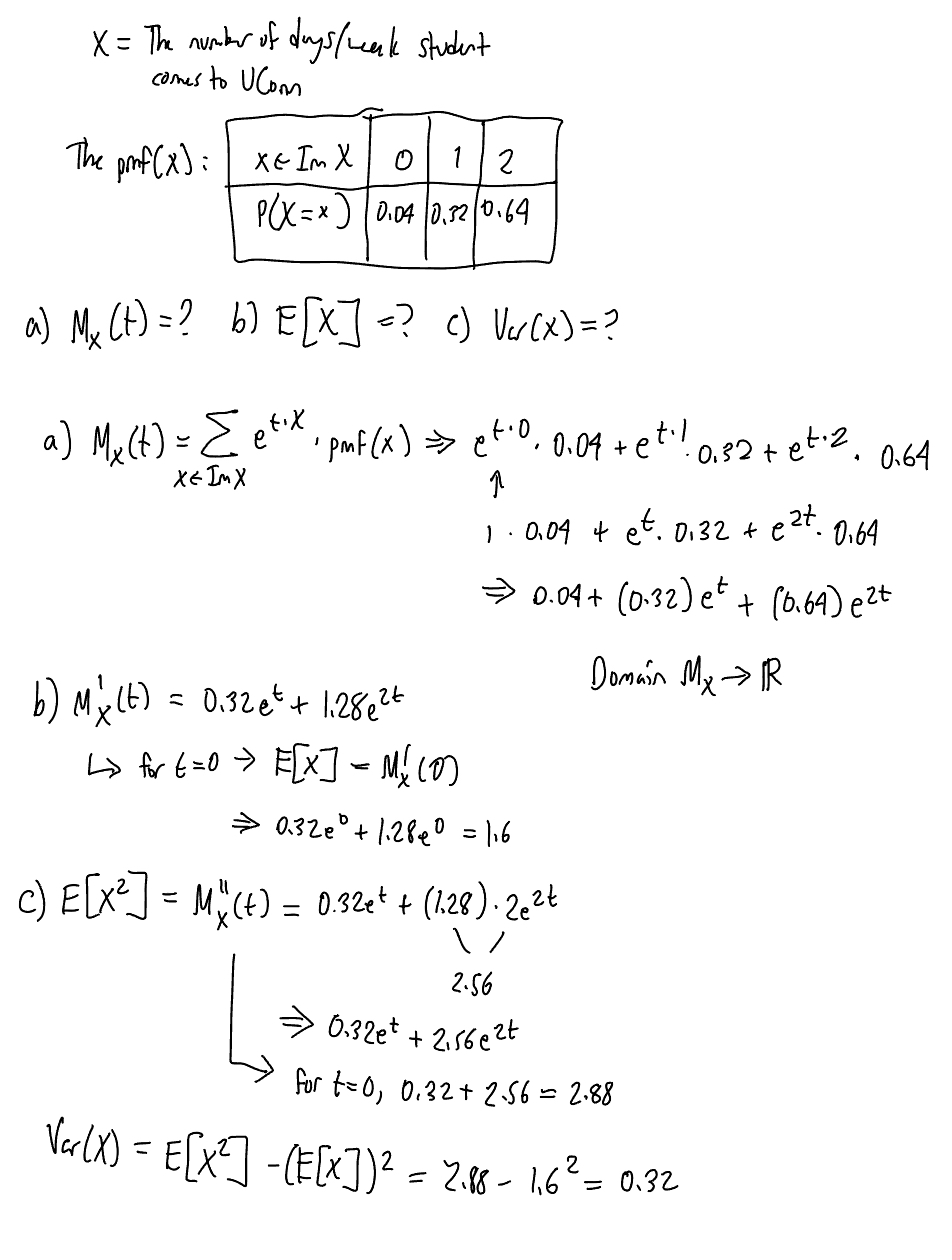
\includegraphics[height=5.5in]{example-mgf.jpeg}

\subsection{The sum of mgf}

There is a property that permits the sum of two independent random variables to be taken with respect to their mgf. Generally speaking, $M_X+M_Y \neq M_{X+Y}$, however, for independent $X$ and $Y$, it holds true. The proof of this property is shown below:

\begin{thm}
    Let $X$ and $Y$ be independent random variables with mgf $M_X(t)$ and $M_Y(t)$, respectively. Then, $M_{X+Y}(t) = M_X(t)M_Y(t)$.
\end{thm}

\begin{proof}
    We will show that given two independent random variables, $X$ and $Y$, the mgf of $X+Y$ is equal to the product of the mgf of $X$ and $Y$. We will do this by showing that the mgf of $X+Y$ is equal to the mgf of $X$ times the mgf of $Y$.

    \begin{align*}
        M_{X+Y}(t) &= E\left[e^{t(X+Y)}\right] \\
        &= E\left[e^{tX} \cdot e^{tY}\right] \\
        &= E\left[e^{tX} \cdot E\left[e^{tY}\right]\right] \\
        &= E\left[e^{tX} \cdot M_Y(t)\right] \\
        &= M_X(t) \cdot M_Y(t)  
    \end{align*}
\end{proof}

\end{document}